\section{More extensions}

  \subsection{Question 1}

In my model, replacing the pump by a better one just means changing the probabilities of PumpFailure (decreasing the probability of failure). 

  \subsection{Question 2}

\textbf{Let} $s = survives$ ; $pfw = pumpFailureWarning$ and $wlw = waterLeakWarning$

$P(s | pfw \lor wlw) = \frac{P(s \land (pfw \lor wlw))}{P(pfw \lor wfw)}
  = \frac{P((s \land pfw) \lor (s \land wlw))}{P(pfw \lor wfw)}$

Or we can easily assume that $WaterLeak$ and $PumpFailure$ are independent and so the warning. \textbf{So :}

$P(s | pfw \lor wlw) = \frac{P(s \land pfw) + P(s \land wlw) - P(s \land pfw \land wlw)}{P(pfw) + p(wlw) - P(pfw)\*P(wlw)}
  = \frac{P(s|pfw)\*P(pfw) + P(s|wlw)\*P(wlw) - P(s|pfw \land wlw)\*P(pfw \land wlw)}{P(pfw) + p(wlw) - P(pfw)\*P(wlw)}$

\textbf{Finally :}

$P(s | pfw \lor wlw)  = \frac{P(s|pfw)\*P(pfw) + P(s|wlw)\*P(wlw) - P(s|pfw \land wlw)\*P(pfw)\*P(wlw)}{P(pfw) + p(wlw) - P(pfw)\*P(wlw)}$

\textbf{The chance of survives is :}
$P(s | pfw \lor wlw)  = \frac{0.96*0.14 + 0.97*0.14 - 0.94*0.14*0.14}{0.14 + 0.14 - 0.14*0.14} = 0.96688$

  \subsection{Question 3}

When we create a Bayesian Network model of a person we restrict the person at a limited set of action which is unrealistic for a person.

  \subsection{Question 4}

To model a more dynamic world where \texttt{IcyWeather} is more likely to be true the next day if it was true the day before we can just chain some \texttt{IcyWeather-X} variables each representing a day. See the figure below.

\begin{figure}[!ht]
  \centering
  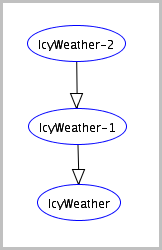
\includegraphics[height=6cm]{img/part4_4.png}
\end{figure} 

